\chapter{METHODOLOGIES AND MODELS}
\thispagestyle{empty}

\section{Conceptual Design}

\subsection{System Architecture Overview}

The proposed recommendation system follows a three-layer pipeline architecture that sequentially transforms raw Wikipedia data into actionable learning paths. Each layer is designed to be modular, allowing independent experimentation and future extension.

\begin{figure}[H]
    \centering
    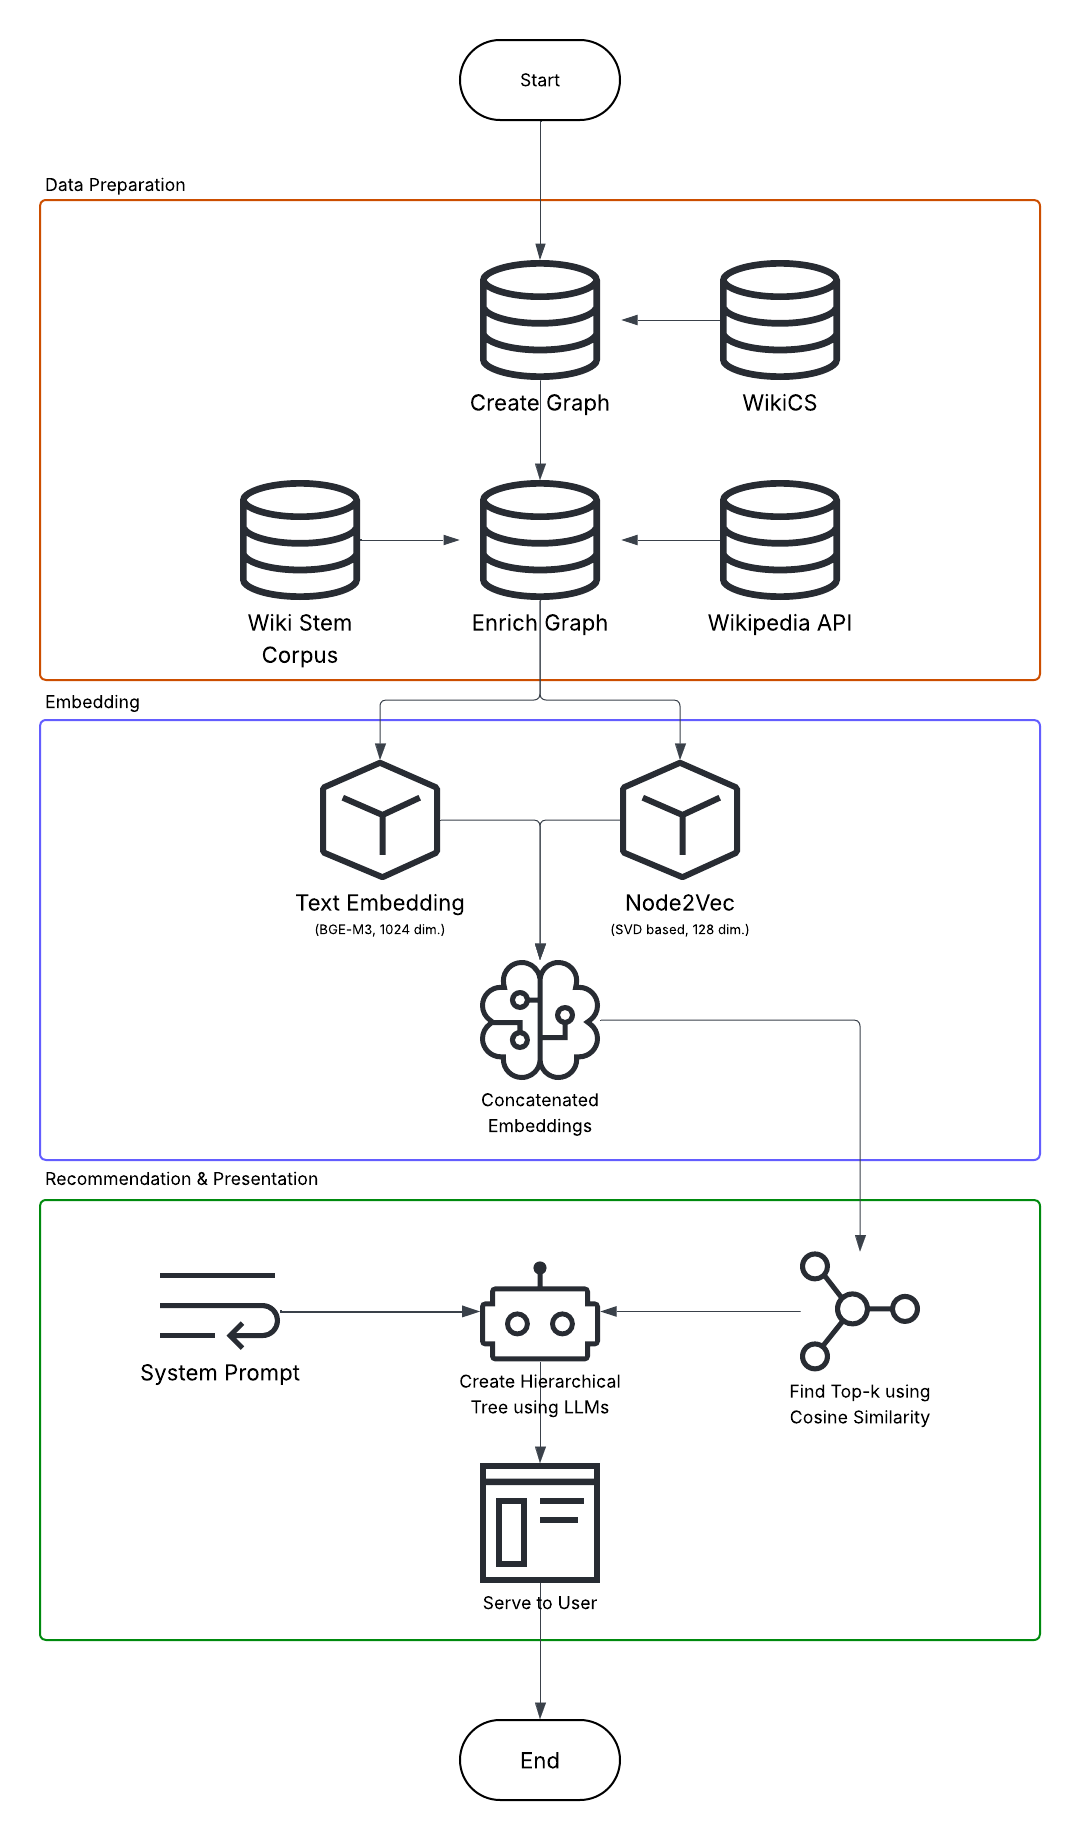
\includegraphics[width=0.75\textwidth]{figures/diagrams/architecture.png}
    \caption{System architecture: three-layer pipeline from Wikipedia data to hierarchical learning paths.}
    \label{fig:system-architecture}
\end{figure}

\textbf{Layer 1 -- Data Preparation:} The WikiCS graph topology is loaded and enriched with article text content fetched via the Wikipedia API. The Wiki Stem Corpus provides supplementary textual data for articles. The resulting graph contains 11,367 nodes (CS articles) and 291,039 directed edges (hyperlinks).

\textbf{Layer 2 -- Embedding:} Two parallel embedding processes are applied to each node. (a) \textit{Text Embedding}: article texts are encoded using BAAI/bge-m3 into 1024-dimensional dense vectors capturing semantic content. (b) \textit{Node2Vec (SVD-based)}: a PPMI matrix factorisation approach produces 128-dimensional structural embeddings reflecting each node's neighbourhood context and graph position. The two vectors are concatenated to form a 1,152-dimensional combined embedding per node, with a degree-normalised popularity penalty applied to the structural component.

\textbf{Layer 3 -- Recommendation and Presentation:} Given a user query, the system encodes the query with the same BGE-M3 model and performs similarity search within the combined text-structural embedding space. The top-$k$ most similar articles are retrieved and passed to a local LLM to generate a hierarchical learning path, which is then served to the user.

\subsection{Data Flow Diagram}

Figure~\ref{fig:data-flow} illustrates the end-to-end data flow from raw Wikipedia data to the final recommendation output. The diagram is structured as two distinct tracks: a \textbf{pre-computed offline track} (top) and a \textbf{query-time online track} (bottom).

\begin{figure}[H]
    \centering
    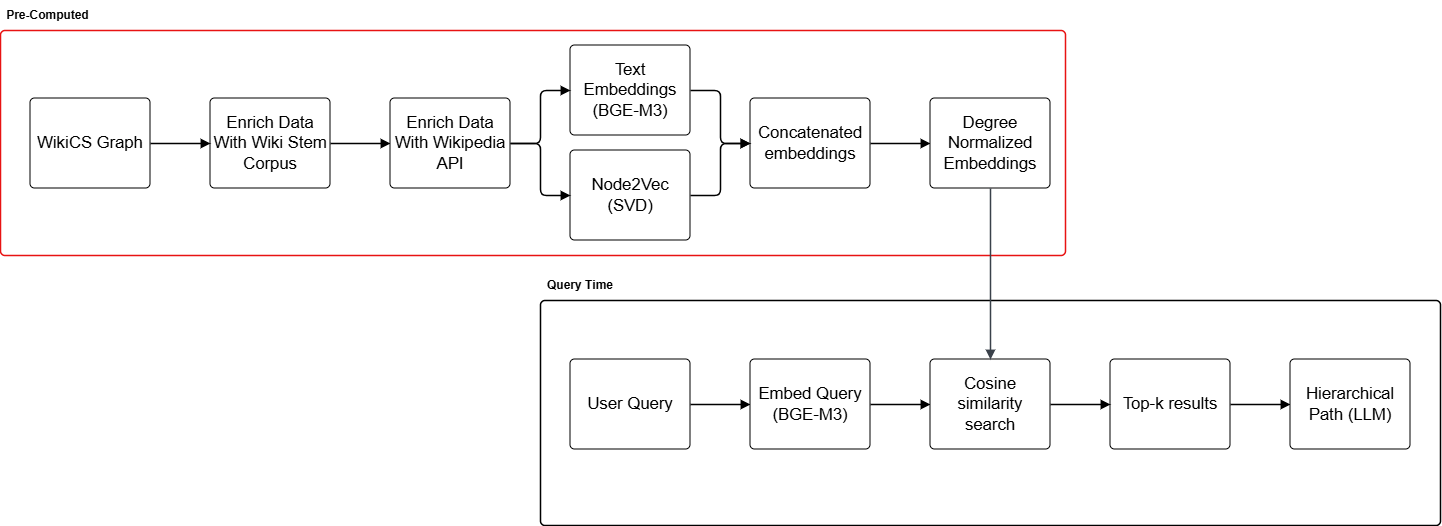
\includegraphics[width=\textwidth]{figures/diagrams/dataflow.png}
    \caption{Data flow diagram: offline pre-computation track (top) and query-time recommendation track (bottom).}
    \label{fig:data-flow}
\end{figure}

\textbf{Offline (Pre-Computed) Track:} This track runs once and caches all results for subsequent queries.
\begin{enumerate}
    \item The WikiCS graph is loaded and enriched with article texts from the Wiki Stem Corpus and the Wikipedia API
    \item Article texts are encoded in parallel via two models: BAAI/bge-m3 (1024-dim text embeddings) and SVD-based Node2Vec (128-dim structural embeddings)
    \item The two embedding vectors are concatenated per node into a 1,152-dim combined representation
    \item A degree-normalised popularity penalty is applied to the structural component, producing the final cached embeddings
\end{enumerate}

\textbf{Query-Time Track:} This track executes in real time for each user query.
\begin{enumerate}
    \item The user submits a topic query string
    \item The query is encoded using the same BAAI/bge-m3 model
    \item The query vector is used to navigate the combined text-structural embedding space, identifying the most semantically relevant articles
    \item The top-$k$ candidates are retrieved and ranked by relevance score
    \item Article titles and metadata are passed to a local LLM, which generates a hierarchical learning path and returns it to the user
\end{enumerate}

\subsection{Interface Mockup}

Figure~\ref{fig:mockup} presents a wireframe of the expected user interface for the recommendation system.

\begin{figure}[H]
    \centering
    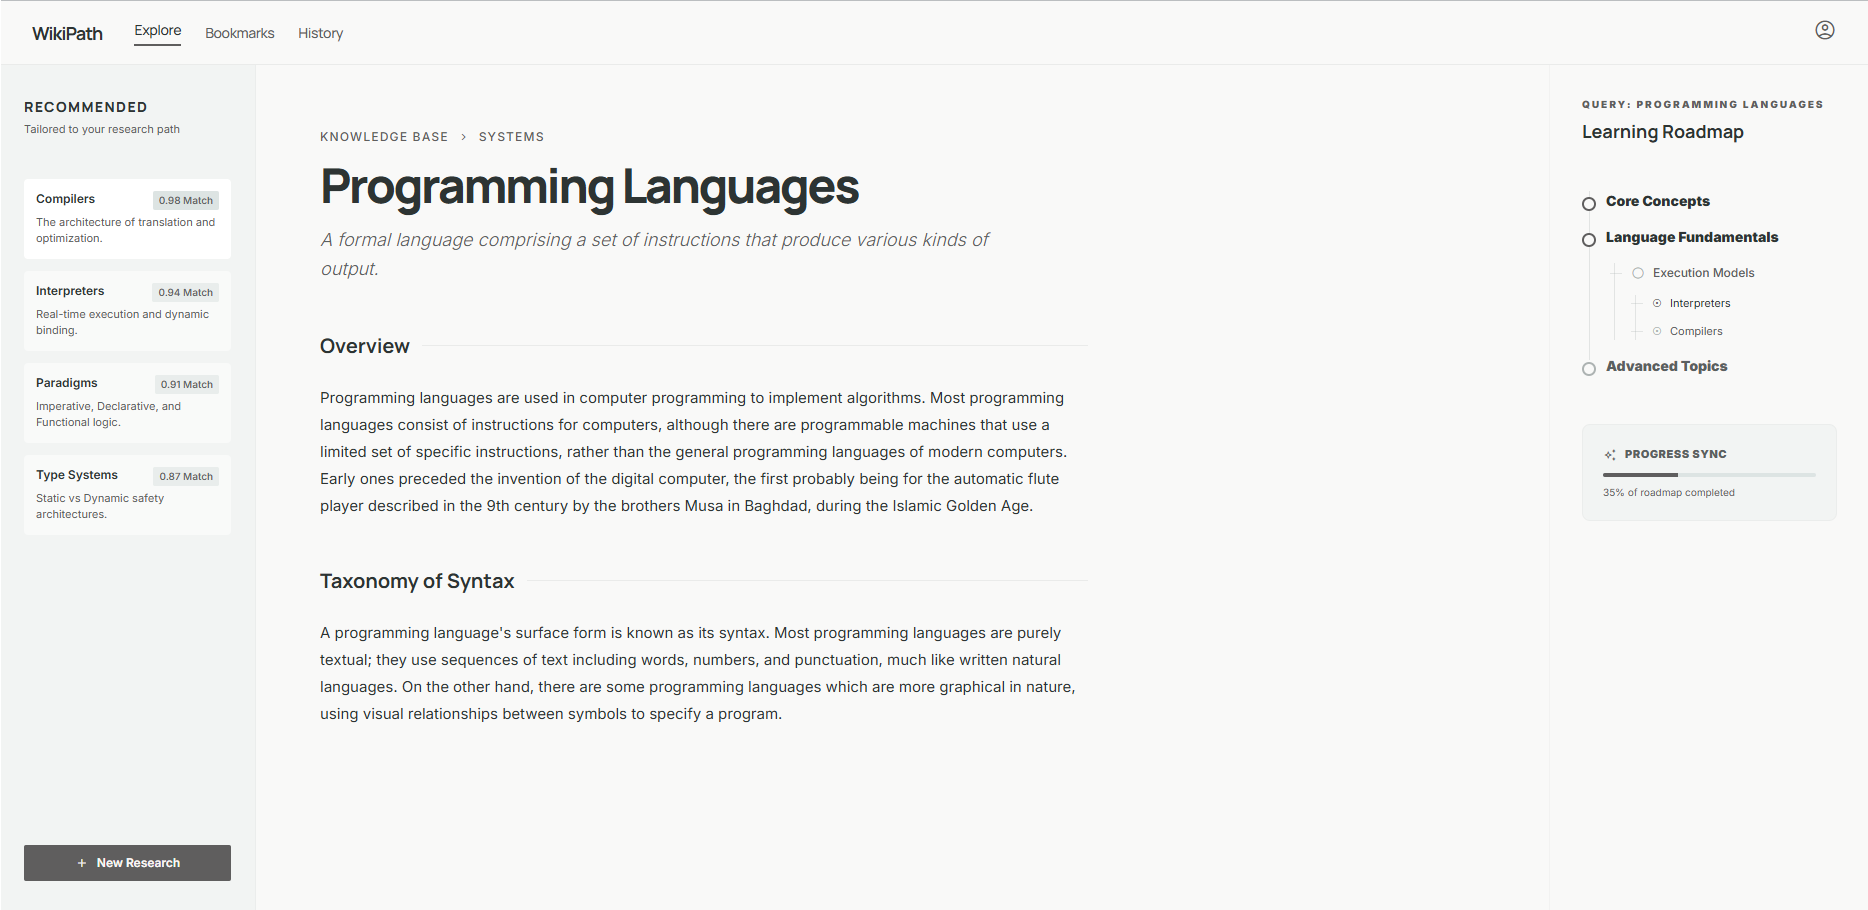
\includegraphics[width=\textwidth]{figures/diagrams/interface-mockup.png}
    \caption{High-fidelity mockup of the WikiPath recommendation interface.}
    \label{fig:mockup}
\end{figure}

The interface follows a three-panel layout:
\begin{itemize}
    \item \textbf{Left panel -- Recommended Articles:} Displays the top-$k$ retrieved articles with their cosine similarity scores (e.g., ``Compilers: 0.98 Match''). Each card includes the article title, a brief description, and a match indicator.
    \item \textbf{Centre panel -- Article View:} Shows the full Wikipedia article content for the currently selected recommendation, including the article title, summary, and sections.
    \item \textbf{Right panel -- Learning Roadmap:} Presents the LLM-generated hierarchical learning path as a collapsible tree (e.g., Core Concepts $\to$ Language Fundamentals $\to$ Execution Models $\to$ Interpreters / Compilers $\to$ Advanced Topics), along with a progress tracker.
\end{itemize}

\subsection{Storyboard: User Journey}

Figure~\ref{fig:storyboard} illustrates the six-step user journey through the WikiPath recommendation system.

\begin{figure}[H]
    \centering
    \includegraphics[width=\textwidth]{figures/diagrams/user-story.png}
    \caption{User journey storyboard: from query entry to hierarchical learning path.}
    \label{fig:storyboard}
\end{figure}

\begin{enumerate}
    \item \textbf{Query Entry:} The user submits a topic query via the search interface (e.g., ``Programming Languages'').
    \item \textbf{Query Encoding:} The query string is encoded into a dense vector using BAAI/bge-m3, producing a 1024-dimensional representation (e.g., $[0.12, -0.74, \ldots]$).
    \item \textbf{Similarity Search:} The encoded query vector is used to navigate the combined text-structural embedding space, identifying the most semantically relevant articles.
    \item \textbf{Candidate Ranking:} Retrieved articles are ranked by similarity score (e.g., Compilers: 0.98, Interpreters: 0.94, Paradigms: 0.91, \ldots).
    \item \textbf{LLM Structuring} \textit{[planned]:} The ranked flat list is passed to a local LLM, which organises the articles into a hierarchical prerequisite structure.
    \item \textbf{Path Presentation} \textit{[planned]:} The final organised hierarchy is displayed to the user as a concept map (e.g., Core Concepts $\to$ Language Fundamentals $\to$ Execution Models $\to$ Compilers / Interpreters).
\end{enumerate}

\section{Technical Design}

\subsection{UML Component Diagram}

Figure~\ref{fig:component-diagram} presents the UML component diagram showing the main software modules and their interactions.

\begin{figure}[H]
    \centering
    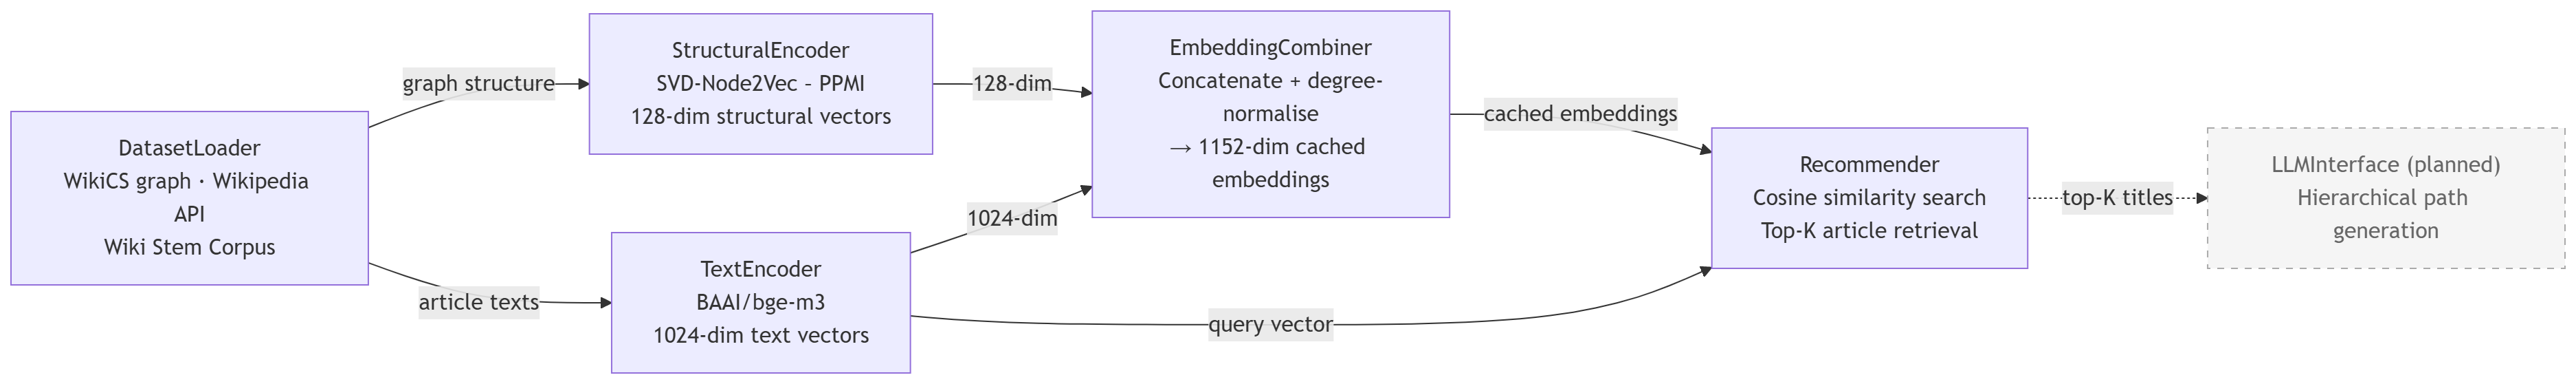
\includegraphics[width=\textwidth]{figures/diagrams/component-diagram.png}
    \caption{UML component diagram of the WikiPath recommendation system.}
    \label{fig:component-diagram}
\end{figure}

The system is decomposed into six components:

\begin{itemize}
    \item \texttt{DatasetLoader:} Loads the WikiCS graph topology and enriches it with article texts retrieved from the Wikipedia API and the Wiki Stem Corpus.
    \item \texttt{TextEncoder:} Wraps BAAI/bge-m3 to encode article texts into 1024-dimensional dense vectors. Also used at query time to encode the user query.
    \item \texttt{StructuralEncoder:} Implements SVD-based Node2Vec via PPMI matrix factorisation, producing 128-dimensional structural embeddings that capture each node's neighbourhood context.
    \item \texttt{EmbeddingCombiner:} Concatenates the 1024-dim text and 128-dim structural vectors into a 1152-dim combined representation, applies a degree-normalised popularity penalty, and caches the result to disk.
    \item \texttt{Recommender:} Encodes the user query using \texttt{TextEncoder} and performs graph-guided similarity search within the cached text-structural embedding space to retrieve the top-$k$ most relevant articles. The exact retrieval strategy is subject to refinement pending supervisor approval.
    \item \texttt{LLMInterface} \textit{(planned):} Will wrap a local LLM served via Ollama to organise the flat top-$k$ list into a hierarchical learning path. Not yet implemented.
\end{itemize}


\subsection{GAT Attention Mechanism}

Graph Attention Networks (GAT) represent a planned future extension of the current pipeline. While the current system uses concatenated BGE-M3 and SVD-based Node2Vec embeddings for recommendations, GAT will be investigated to learn enriched node representations by attending over the hyperlink neighbourhood. The attention mechanism proceeds as follows:

\textbf{Step 1 -- Linear Transformation:} Each node is transformed by a shared learnable weight matrix $\mathbf{W} \in \mathbb{R}^{F' \times F}$:
\[
\vec{h}_i' = \mathbf{W} \vec{h}_i
\]

\textbf{Step 2 -- Attention Coefficient Computation:} The attention coefficient $e_{ij}$ between nodes $i$ and $j$ is computed as:
\[
e_{ij} = \alpha(\mathbf{W}\vec{h}_i, \mathbf{W}\vec{h}_j) = \text{LeakyReLU}\!\left(\vec{a}^T \bigl[\mathbf{W}\vec{h}_i \, || \, \mathbf{W}\vec{h}_j \bigr]\right)
\]
where $\vec{a} \in \mathbb{R}^{2F'}$ is a learnable attention vector and $||$ denotes concatenation.

\textbf{Step 3 -- Normalization:} Attention coefficients are normalized across all neighbors using softmax:
\[
\alpha_{ij} = \text{softmax}_j(e_{ij}) = \frac{\exp(e_{ij})}{\sum_{k \in \mathcal{N}_i} \exp(e_{ik})}
\]

\textbf{Step 4 -- Multi-Head Update:} For stability and capacity, $K$ independent attention heads are used in parallel, and their outputs are averaged (or concatenated):
\[
\vec{h}_i'' = \sigma\!\left(\frac{1}{K} \sum_{k=1}^K \sum_{j \in \mathcal{N}_i} \alpha_{ij}^k \mathbf{W}^k \vec{h}_j \right)
\]

\textbf{Complete GAT Layer:} The full GAT propagation rule is:
\[
\vec{h}_i^{(l+1)} = \sigma\!\left(\sum_{j \in \mathcal{N}_i} \alpha_{ij} \mathbf{W} \vec{h}_j^{(l)}\right)
\]

For a $K$-head GAT layer, the outputs can be concatenated:
\[
\vec{h}_i^{(l+1)} = \bigparallel_{k=1}^K \sigma\!\left(\sum_{j \in \mathcal{N}_i} \alpha_{ij}^k \mathbf{W}^k \vec{h}_j^{(l)}\right)
\]


\section{Experimental Methodology}

\subsection{Dataset: Custom-WikiCS}

The project uses the Custom-WikiCS dataset, a modified version of the Wiki-CS benchmark dataset~\cite{mernyei2020wikics}:

\begin{itemize}
    \item \textbf{Nodes:} 11,367 Wikipedia CS articles (after removing 334 isolated nodes)
    \item \textbf{Directed edges:} 291,039 hyperlinks
    \item \textbf{Undirected edges:} 216,123 (each bidirectional link counted once)
    \item \textbf{Node features:} 1024-dimensional BAAI/bge-m3 embeddings
    \item \textbf{Additional features:} 128-dimensional SVD-based Node2Vec embeddings
\end{itemize}

\subsection{Evaluation Protocol}

The link prediction task follows the standard evaluation protocol:

\begin{itemize}
    \item \textbf{Positive edges:} Existing hyperlinks in the graph
    \item \textbf{Negative edges:} Randomly sampled unconnected node pairs
    \item \textbf{Metrics:} ROC-AUC (Area Under the Receiver Operating Characteristic Curve)
    \item \textbf{Splits:} Per-node 80\% train / 20\% test edge split
\end{itemize}

For the recommendation task:

\begin{itemize}
    \item \textbf{Metrics:} Hits@K (fraction of test neighbors in top-K) and MRR (Mean Reciprocal Rank)
    \item \textbf{Baseline:} Random recommendation (random article selection)
\end{itemize}
